\documentclass[1p]{elsarticle_modified}
%\bibliographystyle{elsarticle-num}

%\usepackage[colorlinks]{hyperref}
%\usepackage{abbrmath_seonhwa} %\Abb, \Ascr, \Acal ,\Abf, \Afrak
\usepackage{amsfonts}
\usepackage{amssymb}
\usepackage{amsmath}
\usepackage{amsthm}
\usepackage{scalefnt}
\usepackage{amsbsy}
\usepackage{kotex}
\usepackage{caption}
\usepackage{subfig}
\usepackage{color}
\usepackage{graphicx}
\usepackage{xcolor} %% white, black, red, green, blue, cyan, magenta, yellow
\usepackage{float}
\usepackage{setspace}
\usepackage{hyperref}

\usepackage{tikz}
\usetikzlibrary{arrows}

\usepackage{multirow}
\usepackage{array} % fixed length table
\usepackage{hhline}

%%%%%%%%%%%%%%%%%%%%%
\makeatletter
\renewcommand*\env@matrix[1][\arraystretch]{%
	\edef\arraystretch{#1}%
	\hskip -\arraycolsep
	\let\@ifnextchar\new@ifnextchar
	\array{*\c@MaxMatrixCols c}}
\makeatother %https://tex.stackexchange.com/questions/14071/how-can-i-increase-the-line-spacing-in-a-matrix
%%%%%%%%%%%%%%%

\usepackage[normalem]{ulem}

\newcommand{\msout}[1]{\ifmmode\text{\sout{\ensuremath{#1}}}\else\sout{#1}\fi}
%SOURCE: \msout is \stkout macro in https://tex.stackexchange.com/questions/20609/strikeout-in-math-mode

\newcommand{\cancel}[1]{
	\ifmmode
	{\color{red}\msout{#1}}
	\else
	{\color{red}\sout{#1}}
	\fi
}

\newcommand{\add}[1]{
	{\color{blue}\uwave{#1}}
}

\newcommand{\replace}[2]{
	\ifmmode
	{\color{red}\msout{#1}}{\color{blue}\uwave{#2}}
	\else
	{\color{red}\sout{#1}}{\color{blue}\uwave{#2}}
	\fi
}

\newcommand{\Sol}{\mathcal{S}} %segment
\newcommand{\D}{D} %diagram
\newcommand{\A}{\mathcal{A}} %arc


%%%%%%%%%%%%%%%%%%%%%%%%%%%%%5 test

\def\sl{\operatorname{\textup{SL}}(2,\Cbb)}
\def\psl{\operatorname{\textup{PSL}}(2,\Cbb)}
\def\quan{\mkern 1mu \triangleright \mkern 1mu}

\theoremstyle{definition}
\newtheorem{thm}{Theorem}[section]
\newtheorem{prop}[thm]{Proposition}
\newtheorem{lem}[thm]{Lemma}
\newtheorem{ques}[thm]{Question}
\newtheorem{cor}[thm]{Corollary}
\newtheorem{defn}[thm]{Definition}
\newtheorem{exam}[thm]{Example}
\newtheorem{rmk}[thm]{Remark}
\newtheorem{alg}[thm]{Algorithm}

\newcommand{\I}{\sqrt{-1}}
\begin{document}

%\begin{frontmatter}
%
%\title{Boundary parabolic representations of knots up to 8 crossings}
%
%%% Group authors per affiliation:
%\author{Yunhi Cho} 
%\address{Department of Mathematics, University of Seoul, Seoul, Korea}
%\ead{yhcho@uos.ac.kr}
%
%
%\author{Seonhwa Kim} %\fnref{s_kim}}
%\address{Center for Geometry and Physics, Institute for Basic Science, Pohang, 37673, Korea}
%\ead{ryeona17@ibs.re.kr}
%
%\author{Hyuk Kim}
%\address{Department of Mathematical Sciences, Seoul National University, Seoul 08826, Korea}
%\ead{hyukkim@snu.ac.kr}
%
%\author{Seokbeom Yoon}
%\address{Department of Mathematical Sciences, Seoul National University, Seoul, 08826,  Korea}
%\ead{sbyoon15@snu.ac.kr}
%
%\begin{abstract}
%We find all boundary parabolic representation of knots up to 8 crossings.
%
%\end{abstract}
%\begin{keyword}
%    \MSC[2010] 57M25 
%\end{keyword}
%
%\end{frontmatter}

%\linenumbers
%\tableofcontents
%
\newcommand\colored[1]{\textcolor{white}{\rule[-0.35ex]{0.8em}{1.4ex}}\kern-0.8em\color{red} #1}%
%\newcommand\colored[1]{\textcolor{white}{ #1}\kern-2.17ex	\textcolor{white}{ #1}\kern-1.81ex	\textcolor{white}{ #1}\kern-2.15ex\color{red}#1	}

{\Large $\underline{12a_{1005}~(K12a_{1005})}$}

\setlength{\tabcolsep}{10pt}
\renewcommand{\arraystretch}{1.6}
\vspace{1cm}\begin{tabular}{m{100pt}>{\centering\arraybackslash}m{274pt}}
\multirow{5}{120pt}{
	\centering
	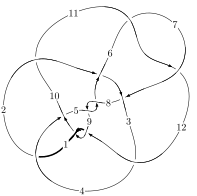
\includegraphics[width=112pt]{../../../GIT/diagram.site/Diagrams/png/1806_12a_1005.png}\\
\ \ \ A knot diagram\footnotemark}&
\allowdisplaybreaks
\textbf{Linearized knot diagam} \\
\cline{2-2}
 &
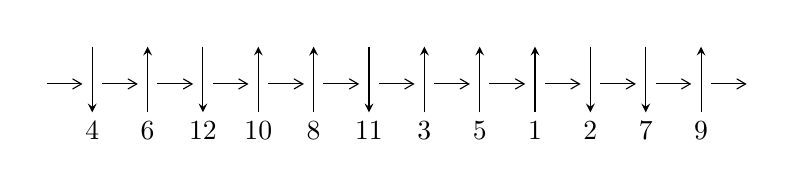
\begin{tikzpicture}[x=20pt, y=17pt]
	% nodes
	\node (C0) at (0, 0) {};
	\node (C1) at (1, 0) {};
	\node (C1U) at (1, +1) {};
	\node (C1D) at (1, -1) {4};

	\node (C2) at (2, 0) {};
	\node (C2U) at (2, +1) {};
	\node (C2D) at (2, -1) {6};

	\node (C3) at (3, 0) {};
	\node (C3U) at (3, +1) {};
	\node (C3D) at (3, -1) {12};

	\node (C4) at (4, 0) {};
	\node (C4U) at (4, +1) {};
	\node (C4D) at (4, -1) {10};

	\node (C5) at (5, 0) {};
	\node (C5U) at (5, +1) {};
	\node (C5D) at (5, -1) {8};

	\node (C6) at (6, 0) {};
	\node (C6U) at (6, +1) {};
	\node (C6D) at (6, -1) {11};

	\node (C7) at (7, 0) {};
	\node (C7U) at (7, +1) {};
	\node (C7D) at (7, -1) {3};

	\node (C8) at (8, 0) {};
	\node (C8U) at (8, +1) {};
	\node (C8D) at (8, -1) {5};

	\node (C9) at (9, 0) {};
	\node (C9U) at (9, +1) {};
	\node (C9D) at (9, -1) {1};

	\node (C10) at (10, 0) {};
	\node (C10U) at (10, +1) {};
	\node (C10D) at (10, -1) {2};

	\node (C11) at (11, 0) {};
	\node (C11U) at (11, +1) {};
	\node (C11D) at (11, -1) {7};

	\node (C12) at (12, 0) {};
	\node (C12U) at (12, +1) {};
	\node (C12D) at (12, -1) {9};
	\node (C13) at (13, 0) {};

	% arrows
	\draw[->,>={angle 60}]
	(C0) edge (C1) (C1) edge (C2) (C2) edge (C3) (C3) edge (C4) (C4) edge (C5) (C5) edge (C6) (C6) edge (C7) (C7) edge (C8) (C8) edge (C9) (C9) edge (C10) (C10) edge (C11) (C11) edge (C12) (C12) edge (C13) ;	\draw[->,>=stealth]
	(C1U) edge (C1D) (C2D) edge (C2U) (C3U) edge (C3D) (C4D) edge (C4U) (C5D) edge (C5U) (C6U) edge (C6D) (C7D) edge (C7U) (C8D) edge (C8U) (C9D) edge (C9U) (C10U) edge (C10D) (C11U) edge (C11D) (C12D) edge (C12U) ;
	\end{tikzpicture} \\
\hhline{~~} \\& 
\textbf{Solving Sequence} \\ \cline{2-2} 
 &
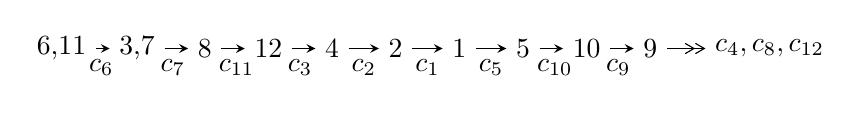
\begin{tikzpicture}[x=23pt, y=7pt]
	% node
	\node (A0) at (-1/8, 0) {6,11};
	\node (A1) at (17/16, 0) {3,7};
	\node (A2) at (17/8, 0) {8};
	\node (A3) at (25/8, 0) {12};
	\node (A4) at (33/8, 0) {4};
	\node (A5) at (41/8, 0) {2};
	\node (A6) at (49/8, 0) {1};
	\node (A7) at (57/8, 0) {5};
	\node (A8) at (65/8, 0) {10};
	\node (A9) at (73/8, 0) {9};
	\node (C1) at (1/2, -1) {$c_{6}$};
	\node (C2) at (13/8, -1) {$c_{7}$};
	\node (C3) at (21/8, -1) {$c_{11}$};
	\node (C4) at (29/8, -1) {$c_{3}$};
	\node (C5) at (37/8, -1) {$c_{2}$};
	\node (C6) at (45/8, -1) {$c_{1}$};
	\node (C7) at (53/8, -1) {$c_{5}$};
	\node (C8) at (61/8, -1) {$c_{10}$};
	\node (C9) at (69/8, -1) {$c_{9}$};
	\node (A10) at (11, 0) {$c_{4},c_{8},c_{12}$};

	% edge
	\draw[->,>=stealth]	
	(A0) edge (A1) (A1) edge (A2) (A2) edge (A3) (A3) edge (A4) (A4) edge (A5) (A5) edge (A6) (A6) edge (A7) (A7) edge (A8) (A8) edge (A9) ;
	\draw[->>,>={angle 60}]	
	(A9) edge (A10);
\end{tikzpicture} \\ 

\end{tabular} \\

\footnotetext{
The image of knot diagram is generated by the software ``\textbf{Draw programme}" developed by Andrew Bartholomew(\url{http://www.layer8.co.uk/maths/draw/index.htm\#Running-draw}), where we modified some parts for our purpose(\url{https://github.com/CATsTAILs/LinksPainter}).
}\phantom \\ \newline 
\centering \textbf{Ideals for irreducible components\footnotemark of $X_{\text{par}}$} 
 
\begin{align*}
I^u_{1}&=\langle 
8.28638\times10^{818} u^{163}+1.07259\times10^{819} u^{162}+\cdots+4.77229\times10^{818} b+8.17270\times10^{819},\\
\phantom{I^u_{1}}&\phantom{= \langle  }8.15374\times10^{819} u^{163}+7.61680\times10^{819} u^{162}+\cdots+4.77229\times10^{818} a+7.02986\times10^{820},\;u^{164}+u^{163}+\cdots+2 u+1\rangle \\
I^u_{2}&=\langle 
-1.98199\times10^{43} u^{43}+9.68400\times10^{42} u^{42}+\cdots+1.94108\times10^{43} b-2.15307\times10^{43},\\
\phantom{I^u_{2}}&\phantom{= \langle  }-8.58634\times10^{42} u^{43}+2.47691\times10^{43} u^{42}+\cdots+1.94108\times10^{43} a-2.23616\times10^{43},\\
\phantom{I^u_{2}}&\phantom{= \langle  }u^{44}-14 u^{42}+\cdots-6 u+1\rangle \\
\\
\end{align*}
\raggedright * 2 irreducible components of $\dim_{\mathbb{C}}=0$, with total 208 representations.\\
\footnotetext{All coefficients of polynomials are rational numbers. But the coefficients are sometimes approximated in decimal forms when there is not enough margin.}
\newpage
\renewcommand{\arraystretch}{1}
\centering \section*{I. $I^u_{1}= \langle 8.29\times10^{818} u^{163}+1.07\times10^{819} u^{162}+\cdots+4.77\times10^{818} b+8.17\times10^{819},\;8.15\times10^{819} u^{163}+7.62\times10^{819} u^{162}+\cdots+4.77\times10^{818} a+7.03\times10^{820},\;u^{164}+u^{163}+\cdots+2 u+1 \rangle$}
\flushleft \textbf{(i) Arc colorings}\\
\begin{tabular}{m{7pt} m{180pt} m{7pt} m{180pt} }
\flushright $a_{6}=$&$\begin{pmatrix}1\\0\end{pmatrix}$ \\
\flushright $a_{11}=$&$\begin{pmatrix}0\\u\end{pmatrix}$ \\
\flushright $a_{3}=$&$\begin{pmatrix}-17.0856 u^{163}-15.9605 u^{162}+\cdots+801.549 u-147.306\\-1.73635 u^{163}-2.24754 u^{162}+\cdots+106.126 u-17.1253\end{pmatrix}$ \\
\flushright $a_{7}=$&$\begin{pmatrix}1\\u^2\end{pmatrix}$ \\
\flushright $a_{8}=$&$\begin{pmatrix}32.9409 u^{163}+27.5908 u^{162}+\cdots-1572.08 u+261.950\\3.86320 u^{163}+2.51080 u^{162}+\cdots-143.117 u+25.0194\end{pmatrix}$ \\
\flushright $a_{12}=$&$\begin{pmatrix}- u\\- u^3+u\end{pmatrix}$ \\
\flushright $a_{4}=$&$\begin{pmatrix}-16.9444 u^{163}-15.4306 u^{162}+\cdots+786.454 u-144.913\\-2.51806 u^{163}-2.41108 u^{162}+\cdots+120.302 u-19.9071\end{pmatrix}$ \\
\flushright $a_{2}=$&$\begin{pmatrix}-15.3492 u^{163}-13.7129 u^{162}+\cdots+695.424 u-130.180\\-1.73635 u^{163}-2.24754 u^{162}+\cdots+106.126 u-17.1253\end{pmatrix}$ \\
\flushright $a_{1}=$&$\begin{pmatrix}29.2656 u^{163}+25.7673 u^{162}+\cdots-1452.79 u+232.311\\1.62972 u^{163}+2.44440 u^{162}+\cdots-147.983 u+21.1918\end{pmatrix}$ \\
\flushright $a_{5}=$&$\begin{pmatrix}11.4222 u^{163}+8.04537 u^{162}+\cdots-456.454 u+83.4972\\1.43923 u^{163}+1.37655 u^{162}+\cdots-71.8732 u+12.2456\end{pmatrix}$ \\
\flushright $a_{10}=$&$\begin{pmatrix}36.6016 u^{163}+33.3168 u^{162}+\cdots-1824.99 u+309.036\\6.11193 u^{163}+3.32962 u^{162}+\cdots-207.355 u+35.1448\end{pmatrix}$ \\
\flushright $a_{9}=$&$\begin{pmatrix}-13.1906 u^{163}-10.9444 u^{162}+\cdots+627.379 u-94.1792\\-1.26477 u^{163}-0.969496 u^{162}+\cdots+57.6793 u-8.49268\end{pmatrix}$\\&\end{tabular}
\flushleft \textbf{(ii) Obstruction class $= -1$}\\~\\
\flushleft \textbf{(iii) Cusp Shapes $= -8.23974 u^{163}-7.66090 u^{162}+\cdots+441.763 u-72.5687$}\\~\\
\newpage\renewcommand{\arraystretch}{1}
\flushleft \textbf{(iv) u-Polynomials at the component}\newline \\
\begin{tabular}{m{50pt}|m{274pt}}
Crossings & \hspace{64pt}u-Polynomials at each crossing \\
\hline $$\begin{aligned}c_{1}\end{aligned}$$&$\begin{aligned}
&u^{164}+5 u^{163}+\cdots-49 u+1
\end{aligned}$\\
\hline $$\begin{aligned}c_{2}\end{aligned}$$&$\begin{aligned}
&u^{164}+u^{163}+\cdots+36157964272 u+1936765232
\end{aligned}$\\
\hline $$\begin{aligned}c_{3}\end{aligned}$$&$\begin{aligned}
&u^{164}-45 u^{162}+\cdots-4066348387 u+426841301
\end{aligned}$\\
\hline $$\begin{aligned}c_{4}\end{aligned}$$&$\begin{aligned}
&u^{164}-2 u^{163}+\cdots+540 u+19
\end{aligned}$\\
\hline $$\begin{aligned}c_{5},c_{8}\end{aligned}$$&$\begin{aligned}
&u^{164}+11 u^{163}+\cdots+9685865 u+827737
\end{aligned}$\\
\hline $$\begin{aligned}c_{6},c_{11}\end{aligned}$$&$\begin{aligned}
&u^{164}- u^{163}+\cdots-2 u+1
\end{aligned}$\\
\hline $$\begin{aligned}c_{7}\end{aligned}$$&$\begin{aligned}
&u^{164}+u^{163}+\cdots+2097860395 u+150897161
\end{aligned}$\\
\hline $$\begin{aligned}c_{9},c_{12}\end{aligned}$$&$\begin{aligned}
&u^{164}-50 u^{162}+\cdots+992 u+1808
\end{aligned}$\\
\hline $$\begin{aligned}c_{10}\end{aligned}$$&$\begin{aligned}
&u^{164}+6 u^{163}+\cdots+1784816067153 u+207574985671
\end{aligned}$\\
\hline
\end{tabular}\\~\\
\newpage\renewcommand{\arraystretch}{1}
\flushleft \textbf{(v) Riley Polynomials at the component}\newline \\
\begin{tabular}{m{50pt}|m{274pt}}
Crossings & \hspace{64pt}Riley Polynomials at each crossing \\
\hline $$\begin{aligned}c_{1}\end{aligned}$$&$\begin{aligned}
&y^{164}+3 y^{163}+\cdots-411 y+1
\end{aligned}$\\
\hline $$\begin{aligned}c_{2}\end{aligned}$$&$\begin{aligned}
&y^{164}+75 y^{163}+\cdots+1.76\times10^{20} y+3.75\times10^{18}
\end{aligned}$\\
\hline $$\begin{aligned}c_{3}\end{aligned}$$&$\begin{aligned}
&y^{164}-90 y^{163}+\cdots-2.04\times10^{19} y+1.82\times10^{17}
\end{aligned}$\\
\hline $$\begin{aligned}c_{4}\end{aligned}$$&$\begin{aligned}
&y^{164}+16 y^{163}+\cdots-4434 y+361
\end{aligned}$\\
\hline $$\begin{aligned}c_{5},c_{8}\end{aligned}$$&$\begin{aligned}
&y^{164}+139 y^{163}+\cdots-8776342483355 y+685148541169
\end{aligned}$\\
\hline $$\begin{aligned}c_{6},c_{11}\end{aligned}$$&$\begin{aligned}
&y^{164}-115 y^{163}+\cdots-170 y+1
\end{aligned}$\\
\hline $$\begin{aligned}c_{7}\end{aligned}$$&$\begin{aligned}
&y^{164}+59 y^{163}+\cdots+634377626274351873 y+22769953197859921
\end{aligned}$\\
\hline $$\begin{aligned}c_{9},c_{12}\end{aligned}$$&$\begin{aligned}
&y^{164}-100 y^{163}+\cdots-153608192 y+3268864
\end{aligned}$\\
\hline $$\begin{aligned}c_{10}\end{aligned}$$&$\begin{aligned}
&y^{164}-108 y^{163}+\cdots-3.42\times10^{24} y+4.31\times10^{22}
\end{aligned}$\\
\hline
\end{tabular}\\~\\
\newpage\flushleft \textbf{(vi) Complex Volumes and Cusp Shapes}
$$\begin{array}{c|c|c}  
\text{Solutions to }I^u_{1}& \I (\text{vol} + \sqrt{-1}CS) & \text{Cusp shape}\\
 \hline 
\begin{aligned}
u &= -0.869177 + 0.509153 I \\
a &= \phantom{-}0.169333 - 1.137160 I \\
b &= -0.342844 - 0.391066 I\end{aligned}
 & \phantom{-}2.88405 - 1.66044 I & \phantom{-0.000000 } 0 \\ \hline\begin{aligned}
u &= -0.869177 - 0.509153 I \\
a &= \phantom{-}0.169333 + 1.137160 I \\
b &= -0.342844 + 0.391066 I\end{aligned}
 & \phantom{-}2.88405 + 1.66044 I & \phantom{-0.000000 } 0 \\ \hline\begin{aligned}
u &= -0.984878 + 0.106592 I \\
a &= -0.98146 + 1.62508 I \\
b &= -0.909765 + 0.456958 I\end{aligned}
 & -5.75041 + 0.39923 I & \phantom{-0.000000 } 0 \\ \hline\begin{aligned}
u &= -0.984878 - 0.106592 I \\
a &= -0.98146 - 1.62508 I \\
b &= -0.909765 - 0.456958 I\end{aligned}
 & -5.75041 - 0.39923 I & \phantom{-0.000000 } 0 \\ \hline\begin{aligned}
u &= -0.989183\phantom{ +0.000000I} \\
a &= \phantom{-}0.323183\phantom{ +0.000000I} \\
b &= \phantom{-}1.49558\phantom{ +0.000000I}\end{aligned}
 & \phantom{-}2.29760\phantom{ +0.000000I} & \phantom{-0.000000 } 0 \\ \hline\begin{aligned}
u &= \phantom{-}0.988638 + 0.009995 I \\
a &= -0.213781 - 0.471004 I \\
b &= -1.34941 - 0.76792 I\end{aligned}
 & -1.65633 + 4.05752 I & \phantom{-0.000000 } 0 \\ \hline\begin{aligned}
u &= \phantom{-}0.988638 - 0.009995 I \\
a &= -0.213781 + 0.471004 I \\
b &= -1.34941 + 0.76792 I\end{aligned}
 & -1.65633 - 4.05752 I & \phantom{-0.000000 } 0 \\ \hline\begin{aligned}
u &= \phantom{-}0.110282 + 1.038000 I \\
a &= -0.409530 - 0.218427 I \\
b &= -0.475993 - 1.080930 I\end{aligned}
 & -4.27505 + 4.09712 I & \phantom{-0.000000 } 0 \\ \hline\begin{aligned}
u &= \phantom{-}0.110282 - 1.038000 I \\
a &= -0.409530 + 0.218427 I \\
b &= -0.475993 + 1.080930 I\end{aligned}
 & -4.27505 - 4.09712 I & \phantom{-0.000000 } 0 \\ \hline\begin{aligned}
u &= \phantom{-}0.568068 + 0.765634 I \\
a &= \phantom{-}0.181874 + 0.180155 I \\
b &= -0.597640 - 0.124843 I\end{aligned}
 & \phantom{-}0.02802 - 2.07677 I & \phantom{-0.000000 } 0\\
 \hline 
 \end{array}$$\newpage$$\begin{array}{c|c|c}  
\text{Solutions to }I^u_{1}& \I (\text{vol} + \sqrt{-1}CS) & \text{Cusp shape}\\
 \hline 
\begin{aligned}
u &= \phantom{-}0.568068 - 0.765634 I \\
a &= \phantom{-}0.181874 - 0.180155 I \\
b &= -0.597640 + 0.124843 I\end{aligned}
 & \phantom{-}0.02802 + 2.07677 I & \phantom{-0.000000 } 0 \\ \hline\begin{aligned}
u &= \phantom{-}0.996494 + 0.342855 I \\
a &= \phantom{-}0.46220 + 1.49178 I \\
b &= -0.299086 + 0.459250 I\end{aligned}
 & -1.37379 - 2.15935 I & \phantom{-0.000000 } 0 \\ \hline\begin{aligned}
u &= \phantom{-}0.996494 - 0.342855 I \\
a &= \phantom{-}0.46220 - 1.49178 I \\
b &= -0.299086 - 0.459250 I\end{aligned}
 & -1.37379 + 2.15935 I & \phantom{-0.000000 } 0 \\ \hline\begin{aligned}
u &= -0.983860 + 0.378927 I \\
a &= \phantom{-}0.82851 - 2.38314 I \\
b &= -0.24401 - 2.23511 I\end{aligned}
 & -1.96890 + 9.67297 I & \phantom{-0.000000 } 0 \\ \hline\begin{aligned}
u &= -0.983860 - 0.378927 I \\
a &= \phantom{-}0.82851 + 2.38314 I \\
b &= -0.24401 + 2.23511 I\end{aligned}
 & -1.96890 - 9.67297 I & \phantom{-0.000000 } 0 \\ \hline\begin{aligned}
u &= \phantom{-}1.000460 + 0.373358 I \\
a &= -0.31736 - 1.74450 I \\
b &= \phantom{-}0.79791 - 1.47090 I\end{aligned}
 & \phantom{-}1.32797 - 6.43845 I & \phantom{-0.000000 } 0 \\ \hline\begin{aligned}
u &= \phantom{-}1.000460 - 0.373358 I \\
a &= -0.31736 + 1.74450 I \\
b &= \phantom{-}0.79791 + 1.47090 I\end{aligned}
 & \phantom{-}1.32797 + 6.43845 I & \phantom{-0.000000 } 0 \\ \hline\begin{aligned}
u &= -0.611311 + 0.879204 I \\
a &= \phantom{-}0.0074746 + 0.0729978 I \\
b &= -0.692411 + 0.111158 I\end{aligned}
 & \phantom{-}3.93629 + 6.69317 I & \phantom{-0.000000 } 0 \\ \hline\begin{aligned}
u &= -0.611311 - 0.879204 I \\
a &= \phantom{-}0.0074746 - 0.0729978 I \\
b &= -0.692411 - 0.111158 I\end{aligned}
 & \phantom{-}3.93629 - 6.69317 I & \phantom{-0.000000 } 0 \\ \hline\begin{aligned}
u &= \phantom{-}0.927110 + 0.008097 I \\
a &= -1.49056 - 2.33101 I \\
b &= -0.60629 - 1.28946 I\end{aligned}
 & -1.38113 + 4.26225 I & \phantom{-0.000000 } 0\\
 \hline 
 \end{array}$$\newpage$$\begin{array}{c|c|c}  
\text{Solutions to }I^u_{1}& \I (\text{vol} + \sqrt{-1}CS) & \text{Cusp shape}\\
 \hline 
\begin{aligned}
u &= \phantom{-}0.927110 - 0.008097 I \\
a &= -1.49056 + 2.33101 I \\
b &= -0.60629 + 1.28946 I\end{aligned}
 & -1.38113 - 4.26225 I & \phantom{-0.000000 } 0 \\ \hline\begin{aligned}
u &= -0.762078 + 0.505620 I \\
a &= \phantom{-}0.465622 - 0.166428 I \\
b &= -0.728178 - 0.821593 I\end{aligned}
 & -4.82240 + 2.94091 I & \phantom{-0.000000 } 0 \\ \hline\begin{aligned}
u &= -0.762078 - 0.505620 I \\
a &= \phantom{-}0.465622 + 0.166428 I \\
b &= -0.728178 + 0.821593 I\end{aligned}
 & -4.82240 - 2.94091 I & \phantom{-0.000000 } 0 \\ \hline\begin{aligned}
u &= \phantom{-}0.121991 + 0.906158 I \\
a &= \phantom{-}0.227372 + 0.611408 I \\
b &= \phantom{-}0.313848 - 1.058270 I\end{aligned}
 & \phantom{-}0.40256 - 2.20922 I & \phantom{-0.000000 } 0 \\ \hline\begin{aligned}
u &= \phantom{-}0.121991 - 0.906158 I \\
a &= \phantom{-}0.227372 - 0.611408 I \\
b &= \phantom{-}0.313848 + 1.058270 I\end{aligned}
 & \phantom{-}0.40256 + 2.20922 I & \phantom{-0.000000 } 0 \\ \hline\begin{aligned}
u &= \phantom{-}0.979536 + 0.479470 I \\
a &= -0.657563 - 0.239774 I \\
b &= -0.886401 - 0.138579 I\end{aligned}
 & -3.26146 - 4.28093 I & \phantom{-0.000000 } 0 \\ \hline\begin{aligned}
u &= \phantom{-}0.979536 - 0.479470 I \\
a &= -0.657563 + 0.239774 I \\
b &= -0.886401 + 0.138579 I\end{aligned}
 & -3.26146 + 4.28093 I & \phantom{-0.000000 } 0 \\ \hline\begin{aligned}
u &= -0.071281 + 0.898521 I \\
a &= \phantom{-}0.420818 + 0.086329 I \\
b &= \phantom{-}0.118209 - 0.746553 I\end{aligned}
 & \phantom{-}1.00223 - 1.62980 I & \phantom{-0.000000 } 0 \\ \hline\begin{aligned}
u &= -0.071281 - 0.898521 I \\
a &= \phantom{-}0.420818 - 0.086329 I \\
b &= \phantom{-}0.118209 + 0.746553 I\end{aligned}
 & \phantom{-}1.00223 + 1.62980 I & \phantom{-0.000000 } 0 \\ \hline\begin{aligned}
u &= \phantom{-}0.524762 + 0.731683 I \\
a &= \phantom{-}0.803081 - 0.246957 I \\
b &= \phantom{-}0.684276 + 0.748128 I\end{aligned}
 & \phantom{-}2.78644 + 2.16616 I & \phantom{-0.000000 } 0\\
 \hline 
 \end{array}$$\newpage$$\begin{array}{c|c|c}  
\text{Solutions to }I^u_{1}& \I (\text{vol} + \sqrt{-1}CS) & \text{Cusp shape}\\
 \hline 
\begin{aligned}
u &= \phantom{-}0.524762 - 0.731683 I \\
a &= \phantom{-}0.803081 + 0.246957 I \\
b &= \phantom{-}0.684276 - 0.748128 I\end{aligned}
 & \phantom{-}2.78644 - 2.16616 I & \phantom{-0.000000 } 0 \\ \hline\begin{aligned}
u &= -0.388899 + 0.789502 I \\
a &= \phantom{-}0.396051 + 0.382103 I \\
b &= -0.666792 + 0.202791 I\end{aligned}
 & \phantom{-}3.92783 - 3.00284 I & \phantom{-0.000000 } 0 \\ \hline\begin{aligned}
u &= -0.388899 - 0.789502 I \\
a &= \phantom{-}0.396051 - 0.382103 I \\
b &= -0.666792 - 0.202791 I\end{aligned}
 & \phantom{-}3.92783 + 3.00284 I & \phantom{-0.000000 } 0 \\ \hline\begin{aligned}
u &= -0.533760 + 0.695751 I \\
a &= -1.166200 + 0.474805 I \\
b &= -0.64659 + 1.32891 I\end{aligned}
 & -0.59796 - 5.44213 I & \phantom{-0.000000 } 0 \\ \hline\begin{aligned}
u &= -0.533760 - 0.695751 I \\
a &= -1.166200 - 0.474805 I \\
b &= -0.64659 - 1.32891 I\end{aligned}
 & -0.59796 + 5.44213 I & \phantom{-0.000000 } 0 \\ \hline\begin{aligned}
u &= \phantom{-}0.510980 + 0.701345 I \\
a &= -0.393768 + 0.930484 I \\
b &= -0.719215 + 0.307785 I\end{aligned}
 & -1.91908 - 0.16586 I & \phantom{-0.000000 } 0 \\ \hline\begin{aligned}
u &= \phantom{-}0.510980 - 0.701345 I \\
a &= -0.393768 - 0.930484 I \\
b &= -0.719215 - 0.307785 I\end{aligned}
 & -1.91908 + 0.16586 I & \phantom{-0.000000 } 0 \\ \hline\begin{aligned}
u &= -0.136828 + 0.854748 I \\
a &= -0.628575 + 0.232734 I \\
b &= \phantom{-}0.934372 - 1.019320 I\end{aligned}
 & -1.107670 + 0.419568 I & \phantom{-0.000000 } 0 \\ \hline\begin{aligned}
u &= -0.136828 - 0.854748 I \\
a &= -0.628575 - 0.232734 I \\
b &= \phantom{-}0.934372 + 1.019320 I\end{aligned}
 & -1.107670 - 0.419568 I & \phantom{-0.000000 } 0 \\ \hline\begin{aligned}
u &= \phantom{-}1.094910 + 0.298629 I \\
a &= \phantom{-}0.20062 - 1.92505 I \\
b &= \phantom{-}0.623344 - 0.958586 I\end{aligned}
 & \phantom{-}2.11373 - 2.89494 I & \phantom{-0.000000 } 0\\
 \hline 
 \end{array}$$\newpage$$\begin{array}{c|c|c}  
\text{Solutions to }I^u_{1}& \I (\text{vol} + \sqrt{-1}CS) & \text{Cusp shape}\\
 \hline 
\begin{aligned}
u &= \phantom{-}1.094910 - 0.298629 I \\
a &= \phantom{-}0.20062 + 1.92505 I \\
b &= \phantom{-}0.623344 + 0.958586 I\end{aligned}
 & \phantom{-}2.11373 + 2.89494 I & \phantom{-0.000000 } 0 \\ \hline\begin{aligned}
u &= -0.042815 + 1.140330 I \\
a &= -0.0374798 - 0.0738951 I \\
b &= \phantom{-}0.630521 + 1.169310 I\end{aligned}
 & -7.07361 + 7.95236 I & \phantom{-0.000000 } 0 \\ \hline\begin{aligned}
u &= -0.042815 - 1.140330 I \\
a &= -0.0374798 + 0.0738951 I \\
b &= \phantom{-}0.630521 - 1.169310 I\end{aligned}
 & -7.07361 - 7.95236 I & \phantom{-0.000000 } 0 \\ \hline\begin{aligned}
u &= \phantom{-}1.144680 + 0.061494 I \\
a &= -0.439003 - 1.032340 I \\
b &= \phantom{-}0.961928 - 0.556071 I\end{aligned}
 & -3.95806 - 1.64685 I & \phantom{-0.000000 } 0 \\ \hline\begin{aligned}
u &= \phantom{-}1.144680 - 0.061494 I \\
a &= -0.439003 + 1.032340 I \\
b &= \phantom{-}0.961928 + 0.556071 I\end{aligned}
 & -3.95806 + 1.64685 I & \phantom{-0.000000 } 0 \\ \hline\begin{aligned}
u &= \phantom{-}1.097070 + 0.341636 I \\
a &= -0.21959 - 2.37665 I \\
b &= \phantom{-}0.724553 - 0.658358 I\end{aligned}
 & -2.31943 - 11.01080 I & \phantom{-0.000000 } 0 \\ \hline\begin{aligned}
u &= \phantom{-}1.097070 - 0.341636 I \\
a &= -0.21959 + 2.37665 I \\
b &= \phantom{-}0.724553 + 0.658358 I\end{aligned}
 & -2.31943 + 11.01080 I & \phantom{-0.000000 } 0 \\ \hline\begin{aligned}
u &= -1.148980 + 0.110231 I \\
a &= \phantom{-}1.88462 - 0.74988 I \\
b &= -0.362477 - 0.523976 I\end{aligned}
 & -8.23855 + 3.87446 I & \phantom{-0.000000 } 0 \\ \hline\begin{aligned}
u &= -1.148980 - 0.110231 I \\
a &= \phantom{-}1.88462 + 0.74988 I \\
b &= -0.362477 + 0.523976 I\end{aligned}
 & -8.23855 - 3.87446 I & \phantom{-0.000000 } 0 \\ \hline\begin{aligned}
u &= -1.084780 + 0.395668 I \\
a &= \phantom{-}0.09976 - 1.59908 I \\
b &= -0.275370 - 0.497316 I\end{aligned}
 & \phantom{-}1.74648 + 7.39363 I & \phantom{-0.000000 } 0\\
 \hline 
 \end{array}$$\newpage$$\begin{array}{c|c|c}  
\text{Solutions to }I^u_{1}& \I (\text{vol} + \sqrt{-1}CS) & \text{Cusp shape}\\
 \hline 
\begin{aligned}
u &= -1.084780 - 0.395668 I \\
a &= \phantom{-}0.09976 + 1.59908 I \\
b &= -0.275370 + 0.497316 I\end{aligned}
 & \phantom{-}1.74648 - 7.39363 I & \phantom{-0.000000 } 0 \\ \hline\begin{aligned}
u &= \phantom{-}0.058061 + 1.156460 I \\
a &= -0.143195 + 0.226079 I \\
b &= -0.382394 + 0.994846 I\end{aligned}
 & -3.78704 - 1.46192 I & \phantom{-0.000000 } 0 \\ \hline\begin{aligned}
u &= \phantom{-}0.058061 - 1.156460 I \\
a &= -0.143195 - 0.226079 I \\
b &= -0.382394 - 0.994846 I\end{aligned}
 & -3.78704 + 1.46192 I & \phantom{-0.000000 } 0 \\ \hline\begin{aligned}
u &= \phantom{-}1.145920 + 0.177078 I \\
a &= -0.57231 + 2.53665 I \\
b &= -1.49586 + 2.26841 I\end{aligned}
 & -7.72342 - 4.92973 I & \phantom{-0.000000 } 0 \\ \hline\begin{aligned}
u &= \phantom{-}1.145920 - 0.177078 I \\
a &= -0.57231 - 2.53665 I \\
b &= -1.49586 - 2.26841 I\end{aligned}
 & -7.72342 + 4.92973 I & \phantom{-0.000000 } 0 \\ \hline\begin{aligned}
u &= -1.161090 + 0.104189 I \\
a &= \phantom{-}2.04318 - 0.94505 I \\
b &= \phantom{-}2.85400 - 1.26008 I\end{aligned}
 & -5.14556 + 9.46016 I & \phantom{-0.000000 } 0 \\ \hline\begin{aligned}
u &= -1.161090 - 0.104189 I \\
a &= \phantom{-}2.04318 + 0.94505 I \\
b &= \phantom{-}2.85400 + 1.26008 I\end{aligned}
 & -5.14556 - 9.46016 I & \phantom{-0.000000 } 0 \\ \hline\begin{aligned}
u &= -1.163070 + 0.091280 I \\
a &= -0.96985 - 2.02725 I \\
b &= -0.004406 - 0.954808 I\end{aligned}
 & -7.49510 + 3.02617 I & \phantom{-0.000000 } 0 \\ \hline\begin{aligned}
u &= -1.163070 - 0.091280 I \\
a &= -0.96985 + 2.02725 I \\
b &= -0.004406 + 0.954808 I\end{aligned}
 & -7.49510 - 3.02617 I & \phantom{-0.000000 } 0 \\ \hline\begin{aligned}
u &= \phantom{-}0.037336 + 1.174070 I \\
a &= \phantom{-}0.0369438 - 0.0021738 I \\
b &= \phantom{-}0.633978 - 1.120670 I\end{aligned}
 & -3.6139 - 14.2988 I & \phantom{-0.000000 } 0\\
 \hline 
 \end{array}$$\newpage$$\begin{array}{c|c|c}  
\text{Solutions to }I^u_{1}& \I (\text{vol} + \sqrt{-1}CS) & \text{Cusp shape}\\
 \hline 
\begin{aligned}
u &= \phantom{-}0.037336 - 1.174070 I \\
a &= \phantom{-}0.0369438 + 0.0021738 I \\
b &= \phantom{-}0.633978 + 1.120670 I\end{aligned}
 & -3.6139 + 14.2988 I & \phantom{-0.000000 } 0 \\ \hline\begin{aligned}
u &= -1.175240 + 0.019483 I \\
a &= -1.08758 - 1.50814 I \\
b &= -1.91459 - 1.19881 I\end{aligned}
 & -6.92293 - 1.18653 I & \phantom{-0.000000 } 0 \\ \hline\begin{aligned}
u &= -1.175240 - 0.019483 I \\
a &= -1.08758 + 1.50814 I \\
b &= -1.91459 + 1.19881 I\end{aligned}
 & -6.92293 + 1.18653 I & \phantom{-0.000000 } 0 \\ \hline\begin{aligned}
u &= \phantom{-}1.177890 + 0.101131 I \\
a &= -0.38284 - 1.39453 I \\
b &= -1.16148 - 1.29798 I\end{aligned}
 & -1.91607 - 5.93788 I & \phantom{-0.000000 } 0 \\ \hline\begin{aligned}
u &= \phantom{-}1.177890 - 0.101131 I \\
a &= -0.38284 + 1.39453 I \\
b &= -1.16148 + 1.29798 I\end{aligned}
 & -1.91607 + 5.93788 I & \phantom{-0.000000 } 0 \\ \hline\begin{aligned}
u &= \phantom{-}0.413597 + 1.111510 I \\
a &= -0.0327605 + 0.0381918 I \\
b &= -0.526517 + 0.780079 I\end{aligned}
 & -3.64684 - 5.55468 I & \phantom{-0.000000 } 0 \\ \hline\begin{aligned}
u &= \phantom{-}0.413597 - 1.111510 I \\
a &= -0.0327605 - 0.0381918 I \\
b &= -0.526517 - 0.780079 I\end{aligned}
 & -3.64684 + 5.55468 I & \phantom{-0.000000 } 0 \\ \hline\begin{aligned}
u &= -1.155270 + 0.298688 I \\
a &= -0.03568 + 1.67083 I \\
b &= \phantom{-}0.81152 + 1.21264 I\end{aligned}
 & -1.86367 + 4.29799 I & \phantom{-0.000000 } 0 \\ \hline\begin{aligned}
u &= -1.155270 - 0.298688 I \\
a &= -0.03568 - 1.67083 I \\
b &= \phantom{-}0.81152 - 1.21264 I\end{aligned}
 & -1.86367 - 4.29799 I & \phantom{-0.000000 } 0 \\ \hline\begin{aligned}
u &= -1.132370 + 0.420585 I \\
a &= -0.42032 + 1.94326 I \\
b &= \phantom{-}1.037530 + 0.744513 I\end{aligned}
 & -4.09090 + 4.18339 I & \phantom{-0.000000 } 0\\
 \hline 
 \end{array}$$\newpage$$\begin{array}{c|c|c}  
\text{Solutions to }I^u_{1}& \I (\text{vol} + \sqrt{-1}CS) & \text{Cusp shape}\\
 \hline 
\begin{aligned}
u &= -1.132370 - 0.420585 I \\
a &= -0.42032 - 1.94326 I \\
b &= \phantom{-}1.037530 - 0.744513 I\end{aligned}
 & -4.09090 - 4.18339 I & \phantom{-0.000000 } 0 \\ \hline\begin{aligned}
u &= \phantom{-}0.387215 + 1.150160 I \\
a &= \phantom{-}0.068647 + 0.367207 I \\
b &= -0.294912 - 0.951769 I\end{aligned}
 & \phantom{-}0.94845 - 2.33153 I & \phantom{-0.000000 } 0 \\ \hline\begin{aligned}
u &= \phantom{-}0.387215 - 1.150160 I \\
a &= \phantom{-}0.068647 - 0.367207 I \\
b &= -0.294912 + 0.951769 I\end{aligned}
 & \phantom{-}0.94845 + 2.33153 I & \phantom{-0.000000 } 0 \\ \hline\begin{aligned}
u &= \phantom{-}1.213060 + 0.091257 I \\
a &= -0.86938 + 1.94522 I \\
b &= \phantom{-}0.097298 + 0.850904 I\end{aligned}
 & -7.35097 + 0.00282 I & \phantom{-0.000000 } 0 \\ \hline\begin{aligned}
u &= \phantom{-}1.213060 - 0.091257 I \\
a &= -0.86938 - 1.94522 I \\
b &= \phantom{-}0.097298 - 0.850904 I\end{aligned}
 & -7.35097 - 0.00282 I & \phantom{-0.000000 } 0 \\ \hline\begin{aligned}
u &= -1.218950 + 0.072910 I \\
a &= -0.332032 + 1.228250 I \\
b &= -0.98997 + 1.05400 I\end{aligned}
 & -5.32723 + 1.90230 I & \phantom{-0.000000 } 0 \\ \hline\begin{aligned}
u &= -1.218950 - 0.072910 I \\
a &= -0.332032 - 1.228250 I \\
b &= -0.98997 - 1.05400 I\end{aligned}
 & -5.32723 - 1.90230 I & \phantom{-0.000000 } 0 \\ \hline\begin{aligned}
u &= -1.213930 + 0.134347 I \\
a &= -0.28497 + 1.49694 I \\
b &= \phantom{-}0.912019 + 0.910189 I\end{aligned}
 & -2.54036 + 6.40960 I & \phantom{-0.000000 } 0 \\ \hline\begin{aligned}
u &= -1.213930 - 0.134347 I \\
a &= -0.28497 - 1.49694 I \\
b &= \phantom{-}0.912019 - 0.910189 I\end{aligned}
 & -2.54036 - 6.40960 I & \phantom{-0.000000 } 0 \\ \hline\begin{aligned}
u &= \phantom{-}1.222810 + 0.019284 I \\
a &= \phantom{-}1.49065 + 1.86983 I \\
b &= \phantom{-}2.20030 + 2.25331 I\end{aligned}
 & -9.54126 - 2.19090 I & \phantom{-0.000000 } 0\\
 \hline 
 \end{array}$$\newpage$$\begin{array}{c|c|c}  
\text{Solutions to }I^u_{1}& \I (\text{vol} + \sqrt{-1}CS) & \text{Cusp shape}\\
 \hline 
\begin{aligned}
u &= \phantom{-}1.222810 - 0.019284 I \\
a &= \phantom{-}1.49065 - 1.86983 I \\
b &= \phantom{-}2.20030 - 2.25331 I\end{aligned}
 & -9.54126 + 2.19090 I & \phantom{-0.000000 } 0 \\ \hline\begin{aligned}
u &= \phantom{-}1.220500 + 0.106731 I \\
a &= \phantom{-}1.58784 + 1.27953 I \\
b &= -0.288614 + 0.645675 I\end{aligned}
 & -6.13373 - 9.45444 I & \phantom{-0.000000 } 0 \\ \hline\begin{aligned}
u &= \phantom{-}1.220500 - 0.106731 I \\
a &= \phantom{-}1.58784 - 1.27953 I \\
b &= -0.288614 - 0.645675 I\end{aligned}
 & -6.13373 + 9.45444 I & \phantom{-0.000000 } 0 \\ \hline\begin{aligned}
u &= -0.282250 + 0.707194 I \\
a &= -0.280043 - 1.165130 I \\
b &= -0.735495 - 0.358113 I\end{aligned}
 & -1.85063 + 2.39683 I & \phantom{-0.000000 } 0 \\ \hline\begin{aligned}
u &= -0.282250 - 0.707194 I \\
a &= -0.280043 + 1.165130 I \\
b &= -0.735495 + 0.358113 I\end{aligned}
 & -1.85063 - 2.39683 I & \phantom{-0.000000 } 0 \\ \hline\begin{aligned}
u &= -1.247330 + 0.058445 I \\
a &= -1.07170 + 1.61991 I \\
b &= -0.067135 + 0.807125 I\end{aligned}
 & -8.55110 - 0.86479 I & \phantom{-0.000000 } 0 \\ \hline\begin{aligned}
u &= -1.247330 - 0.058445 I \\
a &= -1.07170 - 1.61991 I \\
b &= -0.067135 - 0.807125 I\end{aligned}
 & -8.55110 + 0.86479 I & \phantom{-0.000000 } 0 \\ \hline\begin{aligned}
u &= \phantom{-}1.205270 + 0.327362 I \\
a &= \phantom{-}0.669062 + 0.830430 I \\
b &= -0.533111 + 0.808691 I\end{aligned}
 & -3.17488 - 2.14050 I & \phantom{-0.000000 } 0 \\ \hline\begin{aligned}
u &= \phantom{-}1.205270 - 0.327362 I \\
a &= \phantom{-}0.669062 - 0.830430 I \\
b &= -0.533111 - 0.808691 I\end{aligned}
 & -3.17488 + 2.14050 I & \phantom{-0.000000 } 0 \\ \hline\begin{aligned}
u &= \phantom{-}0.327958 + 0.663780 I \\
a &= -0.927633 + 0.038826 I \\
b &= \phantom{-}1.057040 + 0.704387 I\end{aligned}
 & -0.00772 + 7.17049 I & \phantom{-0.000000 } 0\\
 \hline 
 \end{array}$$\newpage$$\begin{array}{c|c|c}  
\text{Solutions to }I^u_{1}& \I (\text{vol} + \sqrt{-1}CS) & \text{Cusp shape}\\
 \hline 
\begin{aligned}
u &= \phantom{-}0.327958 - 0.663780 I \\
a &= -0.927633 - 0.038826 I \\
b &= \phantom{-}1.057040 - 0.704387 I\end{aligned}
 & -0.00772 - 7.17049 I & \phantom{-0.000000 } 0 \\ \hline\begin{aligned}
u &= \phantom{-}0.012202 + 1.265000 I \\
a &= \phantom{-}0.0647472 + 0.0104404 I \\
b &= -0.226588 + 0.775219 I\end{aligned}
 & -1.44674 - 2.78950 I & \phantom{-0.000000 } 0 \\ \hline\begin{aligned}
u &= \phantom{-}0.012202 - 1.265000 I \\
a &= \phantom{-}0.0647472 - 0.0104404 I \\
b &= -0.226588 - 0.775219 I\end{aligned}
 & -1.44674 + 2.78950 I & \phantom{-0.000000 } 0 \\ \hline\begin{aligned}
u &= \phantom{-}1.282870 + 0.113745 I \\
a &= \phantom{-}0.217836 + 1.053510 I \\
b &= -0.458722 + 0.881054 I\end{aligned}
 & -3.27327 - 1.47146 I & \phantom{-0.000000 } 0 \\ \hline\begin{aligned}
u &= \phantom{-}1.282870 - 0.113745 I \\
a &= \phantom{-}0.217836 - 1.053510 I \\
b &= -0.458722 - 0.881054 I\end{aligned}
 & -3.27327 + 1.47146 I & \phantom{-0.000000 } 0 \\ \hline\begin{aligned}
u &= -1.276080 + 0.200277 I \\
a &= -0.343334 + 0.789554 I \\
b &= -0.845919 + 0.569676 I\end{aligned}
 & -5.14547 + 1.35722 I & \phantom{-0.000000 } 0 \\ \hline\begin{aligned}
u &= -1.276080 - 0.200277 I \\
a &= -0.343334 - 0.789554 I \\
b &= -0.845919 - 0.569676 I\end{aligned}
 & -5.14547 - 1.35722 I & \phantom{-0.000000 } 0 \\ \hline\begin{aligned}
u &= \phantom{-}1.314330 + 0.048916 I \\
a &= -0.81780 + 1.67966 I \\
b &= -0.068630 + 0.779887 I\end{aligned}
 & -7.40804 - 4.47819 I & \phantom{-0.000000 } 0 \\ \hline\begin{aligned}
u &= \phantom{-}1.314330 - 0.048916 I \\
a &= -0.81780 - 1.67966 I \\
b &= -0.068630 - 0.779887 I\end{aligned}
 & -7.40804 + 4.47819 I & \phantom{-0.000000 } 0 \\ \hline\begin{aligned}
u &= -0.668100 + 0.128523 I \\
a &= \phantom{-}1.06443 + 1.55537 I \\
b &= \phantom{-}0.475499 + 0.372168 I\end{aligned}
 & \phantom{-}2.64434 + 1.05337 I & \phantom{-0.000000 } 0\\
 \hline 
 \end{array}$$\newpage$$\begin{array}{c|c|c}  
\text{Solutions to }I^u_{1}& \I (\text{vol} + \sqrt{-1}CS) & \text{Cusp shape}\\
 \hline 
\begin{aligned}
u &= -0.668100 - 0.128523 I \\
a &= \phantom{-}1.06443 - 1.55537 I \\
b &= \phantom{-}0.475499 - 0.372168 I\end{aligned}
 & \phantom{-}2.64434 - 1.05337 I & \phantom{-0.000000 } 0 \\ \hline\begin{aligned}
u &= -0.343643 + 0.586130 I \\
a &= \phantom{-}0.207282 + 0.376920 I \\
b &= -0.681941 - 0.905837 I\end{aligned}
 & -4.76926 + 2.89327 I & \phantom{-0.000000 } 0 \\ \hline\begin{aligned}
u &= -0.343643 - 0.586130 I \\
a &= \phantom{-}0.207282 - 0.376920 I \\
b &= -0.681941 + 0.905837 I\end{aligned}
 & -4.76926 - 2.89327 I & \phantom{-0.000000 } 0 \\ \hline\begin{aligned}
u &= -1.325720 + 0.027156 I \\
a &= \phantom{-}0.65965 + 1.59435 I \\
b &= \phantom{-}1.09126 + 1.92199 I\end{aligned}
 & -5.92496 + 5.44183 I & \phantom{-0.000000 } 0 \\ \hline\begin{aligned}
u &= -1.325720 - 0.027156 I \\
a &= \phantom{-}0.65965 - 1.59435 I \\
b &= \phantom{-}1.09126 - 1.92199 I\end{aligned}
 & -5.92496 - 5.44183 I & \phantom{-0.000000 } 0 \\ \hline\begin{aligned}
u &= -1.281900 + 0.498733 I \\
a &= -0.892083 + 0.763089 I \\
b &= \phantom{-}0.117064 + 0.851389 I\end{aligned}
 & -8.57748 + 0.88225 I & \phantom{-0.000000 } 0 \\ \hline\begin{aligned}
u &= -1.281900 - 0.498733 I \\
a &= -0.892083 - 0.763089 I \\
b &= \phantom{-}0.117064 - 0.851389 I\end{aligned}
 & -8.57748 - 0.88225 I & \phantom{-0.000000 } 0 \\ \hline\begin{aligned}
u &= -0.198614 + 0.577381 I \\
a &= \phantom{-}0.239318 + 0.330408 I \\
b &= \phantom{-}0.595695 - 0.486141 I\end{aligned}
 & \phantom{-}1.010920 - 0.883539 I & \phantom{-0.000000 } 0 \\ \hline\begin{aligned}
u &= -0.198614 - 0.577381 I \\
a &= \phantom{-}0.239318 - 0.330408 I \\
b &= \phantom{-}0.595695 + 0.486141 I\end{aligned}
 & \phantom{-}1.010920 + 0.883539 I & \phantom{-0.000000 } 0 \\ \hline\begin{aligned}
u &= \phantom{-}1.323560 + 0.441421 I \\
a &= \phantom{-}0.864050 + 1.015820 I \\
b &= \phantom{-}0.27725 + 1.79614 I\end{aligned}
 & -5.56788 - 5.01333 I & \phantom{-0.000000 } 0\\
 \hline 
 \end{array}$$\newpage$$\begin{array}{c|c|c}  
\text{Solutions to }I^u_{1}& \I (\text{vol} + \sqrt{-1}CS) & \text{Cusp shape}\\
 \hline 
\begin{aligned}
u &= \phantom{-}1.323560 - 0.441421 I \\
a &= \phantom{-}0.864050 - 1.015820 I \\
b &= \phantom{-}0.27725 - 1.79614 I\end{aligned}
 & -5.56788 + 5.01333 I & \phantom{-0.000000 } 0 \\ \hline\begin{aligned}
u &= \phantom{-}0.325093 + 0.508781 I \\
a &= -0.081684 + 0.140427 I \\
b &= \phantom{-}1.006040 + 0.467639 I\end{aligned}
 & \phantom{-}4.45069 - 0.36184 I & \phantom{-0.000000 } 0 \\ \hline\begin{aligned}
u &= \phantom{-}0.325093 - 0.508781 I \\
a &= -0.081684 - 0.140427 I \\
b &= \phantom{-}1.006040 - 0.467639 I\end{aligned}
 & \phantom{-}4.45069 + 0.36184 I & \phantom{-0.000000 } 0 \\ \hline\begin{aligned}
u &= \phantom{-}1.36885 + 0.36876 I \\
a &= -0.04057 + 1.70575 I \\
b &= -0.92514 + 1.54786 I\end{aligned}
 & -9.90194 - 6.89799 I & \phantom{-0.000000 } 0 \\ \hline\begin{aligned}
u &= \phantom{-}1.36885 - 0.36876 I \\
a &= -0.04057 - 1.70575 I \\
b &= -0.92514 - 1.54786 I\end{aligned}
 & -9.90194 + 6.89799 I & \phantom{-0.000000 } 0 \\ \hline\begin{aligned}
u &= -1.33014 + 0.51525 I \\
a &= -0.316409 + 1.292020 I \\
b &= \phantom{-}0.46348 + 1.40607 I\end{aligned}
 & -2.92403 + 6.94331 I & \phantom{-0.000000 } 0 \\ \hline\begin{aligned}
u &= -1.33014 - 0.51525 I \\
a &= -0.316409 - 1.292020 I \\
b &= \phantom{-}0.46348 - 1.40607 I\end{aligned}
 & -2.92403 - 6.94331 I & \phantom{-0.000000 } 0 \\ \hline\begin{aligned}
u &= \phantom{-}1.34450 + 0.53734 I \\
a &= \phantom{-}0.27958 + 1.63896 I \\
b &= -0.59477 + 1.49157 I\end{aligned}
 & -8.21494 - 9.81676 I & \phantom{-0.000000 } 0 \\ \hline\begin{aligned}
u &= \phantom{-}1.34450 - 0.53734 I \\
a &= \phantom{-}0.27958 - 1.63896 I \\
b &= -0.59477 - 1.49157 I\end{aligned}
 & -8.21494 + 9.81676 I & \phantom{-0.000000 } 0 \\ \hline\begin{aligned}
u &= -0.00921 + 1.45579 I \\
a &= -0.0124504 + 0.0153640 I \\
b &= -0.243685 - 0.693284 I\end{aligned}
 & \phantom{-}2.54879 + 6.99583 I & \phantom{-0.000000 } 0\\
 \hline 
 \end{array}$$\newpage$$\begin{array}{c|c|c}  
\text{Solutions to }I^u_{1}& \I (\text{vol} + \sqrt{-1}CS) & \text{Cusp shape}\\
 \hline 
\begin{aligned}
u &= -0.00921 - 1.45579 I \\
a &= -0.0124504 - 0.0153640 I \\
b &= -0.243685 + 0.693284 I\end{aligned}
 & \phantom{-}2.54879 - 6.99583 I & \phantom{-0.000000 } 0 \\ \hline\begin{aligned}
u &= \phantom{-}1.35734 + 0.56356 I \\
a &= \phantom{-}0.321951 + 1.046950 I \\
b &= -0.830586 + 1.050930 I\end{aligned}
 & -2.53664 - 3.87888 I & \phantom{-0.000000 } 0 \\ \hline\begin{aligned}
u &= \phantom{-}1.35734 - 0.56356 I \\
a &= \phantom{-}0.321951 - 1.046950 I \\
b &= -0.830586 - 1.050930 I\end{aligned}
 & -2.53664 + 3.87888 I & \phantom{-0.000000 } 0 \\ \hline\begin{aligned}
u &= -1.40589 + 0.47370 I \\
a &= -0.21826 + 1.60316 I \\
b &= \phantom{-}1.18111 + 2.01498 I\end{aligned}
 & -4.50560 + 7.27936 I & \phantom{-0.000000 } 0 \\ \hline\begin{aligned}
u &= -1.40589 - 0.47370 I \\
a &= -0.21826 - 1.60316 I \\
b &= \phantom{-}1.18111 - 2.01498 I\end{aligned}
 & -4.50560 - 7.27936 I & \phantom{-0.000000 } 0 \\ \hline\begin{aligned}
u &= \phantom{-}1.38998 + 0.52477 I \\
a &= -0.22510 - 1.59400 I \\
b &= \phantom{-}1.05072 - 1.52408 I\end{aligned}
 & -11.6002 - 13.7978 I & \phantom{-0.000000 } 0 \\ \hline\begin{aligned}
u &= \phantom{-}1.38998 - 0.52477 I \\
a &= -0.22510 + 1.59400 I \\
b &= \phantom{-}1.05072 + 1.52408 I\end{aligned}
 & -11.6002 + 13.7978 I & \phantom{-0.000000 } 0 \\ \hline\begin{aligned}
u &= -1.40616 + 0.50944 I \\
a &= \phantom{-}0.25369 - 1.53815 I \\
b &= -0.64117 - 1.36346 I\end{aligned}
 & -8.47222 + 7.31099 I & \phantom{-0.000000 } 0 \\ \hline\begin{aligned}
u &= -1.40616 - 0.50944 I \\
a &= \phantom{-}0.25369 + 1.53815 I \\
b &= -0.64117 + 1.36346 I\end{aligned}
 & -8.47222 - 7.31099 I & \phantom{-0.000000 } 0 \\ \hline\begin{aligned}
u &= -1.43705 + 0.41795 I \\
a &= -0.02431 - 1.53046 I \\
b &= -0.90783 - 1.39477 I\end{aligned}
 & -9.3423 + 10.7264 I & \phantom{-0.000000 } 0\\
 \hline 
 \end{array}$$\newpage$$\begin{array}{c|c|c}  
\text{Solutions to }I^u_{1}& \I (\text{vol} + \sqrt{-1}CS) & \text{Cusp shape}\\
 \hline 
\begin{aligned}
u &= -1.43705 - 0.41795 I \\
a &= -0.02431 + 1.53046 I \\
b &= -0.90783 + 1.39477 I\end{aligned}
 & -9.3423 - 10.7264 I & \phantom{-0.000000 } 0 \\ \hline\begin{aligned}
u &= -1.39920 + 0.53936 I \\
a &= -0.20694 + 1.58779 I \\
b &= \phantom{-}0.99308 + 1.50160 I\end{aligned}
 & -8.1548 + 20.2998 I & \phantom{-0.000000 } 0 \\ \hline\begin{aligned}
u &= -1.39920 - 0.53936 I \\
a &= -0.20694 - 1.58779 I \\
b &= \phantom{-}0.99308 - 1.50160 I\end{aligned}
 & -8.1548 - 20.2998 I & \phantom{-0.000000 } 0 \\ \hline\begin{aligned}
u &= -1.42181 + 0.53107 I \\
a &= \phantom{-}0.173019 - 1.208400 I \\
b &= -0.817042 - 1.134700 I\end{aligned}
 & -6.16542 + 9.00087 I & \phantom{-0.000000 } 0 \\ \hline\begin{aligned}
u &= -1.42181 - 0.53107 I \\
a &= \phantom{-}0.173019 + 1.208400 I \\
b &= -0.817042 + 1.134700 I\end{aligned}
 & -6.16542 - 9.00087 I & \phantom{-0.000000 } 0 \\ \hline\begin{aligned}
u &= \phantom{-}1.41936 + 0.55478 I \\
a &= -0.611534 - 0.893951 I \\
b &= \phantom{-}0.162081 - 0.978837 I\end{aligned}
 & -8.13440 - 4.73588 I & \phantom{-0.000000 } 0 \\ \hline\begin{aligned}
u &= \phantom{-}1.41936 - 0.55478 I \\
a &= -0.611534 + 0.893951 I \\
b &= \phantom{-}0.162081 + 0.978837 I\end{aligned}
 & -8.13440 + 4.73588 I & \phantom{-0.000000 } 0 \\ \hline\begin{aligned}
u &= \phantom{-}1.45901 + 0.49891 I \\
a &= -0.199424 - 1.013340 I \\
b &= \phantom{-}0.478238 - 1.119680 I\end{aligned}
 & -6.38776 - 3.51668 I & \phantom{-0.000000 } 0 \\ \hline\begin{aligned}
u &= \phantom{-}1.45901 - 0.49891 I \\
a &= -0.199424 + 1.013340 I \\
b &= \phantom{-}0.478238 + 1.119680 I\end{aligned}
 & -6.38776 + 3.51668 I & \phantom{-0.000000 } 0 \\ \hline\begin{aligned}
u &= -1.44500 + 0.54637 I \\
a &= \phantom{-}0.599728 - 0.761273 I \\
b &= -0.075661 - 1.248430 I\end{aligned}
 & -11.49990 - 1.75481 I & \phantom{-0.000000 } 0\\
 \hline 
 \end{array}$$\newpage$$\begin{array}{c|c|c}  
\text{Solutions to }I^u_{1}& \I (\text{vol} + \sqrt{-1}CS) & \text{Cusp shape}\\
 \hline 
\begin{aligned}
u &= -1.44500 - 0.54637 I \\
a &= \phantom{-}0.599728 + 0.761273 I \\
b &= -0.075661 + 1.248430 I\end{aligned}
 & -11.49990 + 1.75481 I & \phantom{-0.000000 } 0 \\ \hline\begin{aligned}
u &= \phantom{-}1.45510 + 0.55770 I \\
a &= \phantom{-}0.062544 + 1.158230 I \\
b &= -0.88196 + 1.12725 I\end{aligned}
 & -2.38417 - 13.73050 I & \phantom{-0.000000 } 0 \\ \hline\begin{aligned}
u &= \phantom{-}1.45510 - 0.55770 I \\
a &= \phantom{-}0.062544 - 1.158230 I \\
b &= -0.88196 - 1.12725 I\end{aligned}
 & -2.38417 + 13.73050 I & \phantom{-0.000000 } 0 \\ \hline\begin{aligned}
u &= \phantom{-}1.49488 + 0.54971 I \\
a &= \phantom{-}0.556075 + 0.702569 I \\
b &= -0.074312 + 1.106710 I\end{aligned}
 & -8.20067 + 7.88855 I & \phantom{-0.000000 } 0 \\ \hline\begin{aligned}
u &= \phantom{-}1.49488 - 0.54971 I \\
a &= \phantom{-}0.556075 - 0.702569 I \\
b &= -0.074312 - 1.106710 I\end{aligned}
 & -8.20067 - 7.88855 I & \phantom{-0.000000 } 0 \\ \hline\begin{aligned}
u &= -1.54678 + 0.38241 I \\
a &= \phantom{-}0.058988 + 0.963652 I \\
b &= \phantom{-}0.671602 + 1.051840 I\end{aligned}
 & -3.44852 - 0.15850 I & \phantom{-0.000000 } 0 \\ \hline\begin{aligned}
u &= -1.54678 - 0.38241 I \\
a &= \phantom{-}0.058988 - 0.963652 I \\
b &= \phantom{-}0.671602 - 1.051840 I\end{aligned}
 & -3.44852 + 0.15850 I & \phantom{-0.000000 } 0 \\ \hline\begin{aligned}
u &= -0.403651\phantom{ +0.000000I} \\
a &= \phantom{-}0.269102\phantom{ +0.000000I} \\
b &= \phantom{-}1.17376\phantom{ +0.000000I}\end{aligned}
 & \phantom{-}3.11032\phantom{ +0.000000I} & -14.4860\phantom{ +0.000000I} \\ \hline\begin{aligned}
u &= -0.017309 + 0.345215 I \\
a &= -0.64237 + 1.75395 I \\
b &= -0.754075 - 0.974867 I\end{aligned}
 & -4.65307 + 2.82812 I & -1.91627 - 3.18964 I \\ \hline\begin{aligned}
u &= -0.017309 - 0.345215 I \\
a &= -0.64237 - 1.75395 I \\
b &= -0.754075 + 0.974867 I\end{aligned}
 & -4.65307 - 2.82812 I & -1.91627 + 3.18964 I\\
 \hline 
 \end{array}$$\newpage$$\begin{array}{c|c|c}  
\text{Solutions to }I^u_{1}& \I (\text{vol} + \sqrt{-1}CS) & \text{Cusp shape}\\
 \hline 
\begin{aligned}
u &= -1.46816 + 0.88855 I \\
a &= -0.331077 + 0.392184 I \\
b &= \phantom{-}0.298333 + 0.738138 I\end{aligned}
 & -6.28229 + 4.32405 I & \phantom{-0.000000 } 0 \\ \hline\begin{aligned}
u &= -1.46816 - 0.88855 I \\
a &= -0.331077 - 0.392184 I \\
b &= \phantom{-}0.298333 - 0.738138 I\end{aligned}
 & -6.28229 - 4.32405 I & \phantom{-0.000000 } 0 \\ \hline\begin{aligned}
u &= \phantom{-}1.58743 + 0.69474 I \\
a &= -0.213989 - 0.594570 I \\
b &= \phantom{-}0.414341 - 0.814522 I\end{aligned}
 & -7.00010 - 2.20644 I & \phantom{-0.000000 } 0 \\ \hline\begin{aligned}
u &= \phantom{-}1.58743 - 0.69474 I \\
a &= -0.213989 + 0.594570 I \\
b &= \phantom{-}0.414341 + 0.814522 I\end{aligned}
 & -7.00010 + 2.20644 I & \phantom{-0.000000 } 0 \\ \hline\begin{aligned}
u &= -0.156395 + 0.203509 I \\
a &= -0.57502 - 5.54669 I \\
b &= \phantom{-}0.577216 + 0.859044 I\end{aligned}
 & -5.50574 - 2.51494 I & -0.277428 + 1.330396 I \\ \hline\begin{aligned}
u &= -0.156395 - 0.203509 I \\
a &= -0.57502 + 5.54669 I \\
b &= \phantom{-}0.577216 - 0.859044 I\end{aligned}
 & -5.50574 + 2.51494 I & -0.277428 - 1.330396 I \\ \hline\begin{aligned}
u &= \phantom{-}0.172907 + 0.041641 I \\
a &= \phantom{-}5.13888 + 1.21083 I \\
b &= -0.051203 - 0.483822 I\end{aligned}
 & -1.37595 - 1.18765 I & -5.19575 - 0.40054 I \\ \hline\begin{aligned}
u &= \phantom{-}0.172907 - 0.041641 I \\
a &= \phantom{-}5.13888 - 1.21083 I \\
b &= -0.051203 + 0.483822 I\end{aligned}
 & -1.37595 + 1.18765 I & -5.19575 + 0.40054 I \\ \hline\begin{aligned}
u &= -0.0350083 + 0.1355980 I \\
a &= -0.33266 - 7.16426 I \\
b &= -0.679654 - 0.787469 I\end{aligned}
 & -3.73207 - 1.00515 I & -2.40866 + 2.83393 I \\ \hline\begin{aligned}
u &= -0.0350083 - 0.1355980 I \\
a &= -0.33266 + 7.16426 I \\
b &= -0.679654 + 0.787469 I\end{aligned}
 & -3.73207 + 1.00515 I & -2.40866 - 2.83393 I\\
 \hline 
 \end{array}$$\newpage$$\begin{array}{c|c|c}  
\text{Solutions to }I^u_{1}& \I (\text{vol} + \sqrt{-1}CS) & \text{Cusp shape}\\
 \hline 
\begin{aligned}
u &= -0.1232550 + 0.0012074 I \\
a &= \phantom{-}10.42810 - 7.79652 I \\
b &= \phantom{-}0.794455 - 0.940532 I\end{aligned}
 & -2.25570 + 8.60093 I & \phantom{-}2.87789 - 3.87010 I \\ \hline\begin{aligned}
u &= -0.1232550 - 0.0012074 I \\
a &= \phantom{-}10.42810 + 7.79652 I \\
b &= \phantom{-}0.794455 + 0.940532 I\end{aligned}
 & -2.25570 - 8.60093 I & \phantom{-}2.87789 + 3.87010 I \\ \hline\begin{aligned}
u &= \phantom{-}0.0779976 + 0.0571355 I \\
a &= -11.07950 - 0.60969 I \\
b &= \phantom{-}0.081061 - 0.855623 I\end{aligned}
 & \phantom{-}1.20762 - 5.23630 I & -0.16932 + 5.08837 I \\ \hline\begin{aligned}
u &= \phantom{-}0.0779976 - 0.0571355 I \\
a &= -11.07950 + 0.60969 I \\
b &= \phantom{-}0.081061 + 0.855623 I\end{aligned}
 & \phantom{-}1.20762 + 5.23630 I & -0.16932 - 5.08837 I\\
 \hline 
 \end{array}$$\newpage\newpage\renewcommand{\arraystretch}{1}
\centering \section*{II. $I^u_{2}= \langle -1.98\times10^{43} u^{43}+9.68\times10^{42} u^{42}+\cdots+1.94\times10^{43} b-2.15\times10^{43},\;-8.59\times10^{42} u^{43}+2.48\times10^{43} u^{42}+\cdots+1.94\times10^{43} a-2.24\times10^{43},\;u^{44}-14 u^{42}+\cdots-6 u+1 \rangle$}
\flushleft \textbf{(i) Arc colorings}\\
\begin{tabular}{m{7pt} m{180pt} m{7pt} m{180pt} }
\flushright $a_{6}=$&$\begin{pmatrix}1\\0\end{pmatrix}$ \\
\flushright $a_{11}=$&$\begin{pmatrix}0\\u\end{pmatrix}$ \\
\flushright $a_{3}=$&$\begin{pmatrix}0.442348 u^{43}-1.27605 u^{42}+\cdots+9.48823 u+1.15202\\1.02107 u^{43}-0.498897 u^{42}+\cdots+0.456345 u+1.10921\end{pmatrix}$ \\
\flushright $a_{7}=$&$\begin{pmatrix}1\\u^2\end{pmatrix}$ \\
\flushright $a_{8}=$&$\begin{pmatrix}-1.86583 u^{43}+1.94186 u^{42}+\cdots+8.11038 u-2.61443\\-2.73749 u^{43}-1.19751 u^{42}+\cdots-3.68047 u-0.277328\end{pmatrix}$ \\
\flushright $a_{12}=$&$\begin{pmatrix}- u\\- u^3+u\end{pmatrix}$ \\
\flushright $a_{4}=$&$\begin{pmatrix}-0.951559 u^{43}-1.50839 u^{42}+\cdots+9.19417 u+1.36164\\0.530214 u^{43}-0.642325 u^{42}+\cdots+0.750293 u+1.13192\end{pmatrix}$ \\
\flushright $a_{2}=$&$\begin{pmatrix}-0.578727 u^{43}-0.777152 u^{42}+\cdots+9.03189 u+0.0428080\\1.02107 u^{43}-0.498897 u^{42}+\cdots+0.456345 u+1.10921\end{pmatrix}$ \\
\flushright $a_{1}=$&$\begin{pmatrix}3.75965 u^{43}+3.18740 u^{42}+\cdots+26.6527 u+0.527639\\-1.21929 u^{43}-1.45127 u^{42}+\cdots-0.893534 u+3.25217\end{pmatrix}$ \\
\flushright $a_{5}=$&$\begin{pmatrix}-3.03093 u^{43}+0.485290 u^{42}+\cdots+15.7037 u+1.16313\\-1.74433 u^{43}-1.39069 u^{42}+\cdots-0.604828 u+1.79368\end{pmatrix}$ \\
\flushright $a_{10}=$&$\begin{pmatrix}3.10216 u^{43}+1.98381 u^{42}+\cdots+12.5978 u-2.70383\\-0.469843 u^{43}-3.60173 u^{42}+\cdots-13.2327 u+2.48958\end{pmatrix}$ \\
\flushright $a_{9}=$&$\begin{pmatrix}-1.99045 u^{43}-2.99452 u^{42}+\cdots-24.8396 u-1.21104\\0.872695 u^{43}-0.591305 u^{42}+\cdots-6.80976 u-1.68244\end{pmatrix}$\\&\end{tabular}
\flushleft \textbf{(ii) Obstruction class $= 1$}\\~\\
\flushleft \textbf{(iii) Cusp Shapes $= 8.44648 u^{43}+7.77679 u^{42}+\cdots+29.5073 u+7.06652$}\\~\\
\newpage\renewcommand{\arraystretch}{1}
\flushleft \textbf{(iv) u-Polynomials at the component}\newline \\
\begin{tabular}{m{50pt}|m{274pt}}
Crossings & \hspace{64pt}u-Polynomials at each crossing \\
\hline $$\begin{aligned}c_{1}\end{aligned}$$&$\begin{aligned}
&u^{44}-16 u^{43}+\cdots- u+1
\end{aligned}$\\
\hline $$\begin{aligned}c_{2}\end{aligned}$$&$\begin{aligned}
&u^{44}+11 u^{42}+\cdots+24 u+4
\end{aligned}$\\
\hline $$\begin{aligned}c_{3}\end{aligned}$$&$\begin{aligned}
&u^{44}-5 u^{43}+\cdots+459 u+53
\end{aligned}$\\
\hline $$\begin{aligned}c_{4}\end{aligned}$$&$\begin{aligned}
&u^{44}- u^{43}+\cdots-12 u+1
\end{aligned}$\\
\hline $$\begin{aligned}c_{5}\end{aligned}$$&$\begin{aligned}
&u^{44}+2 u^{43}+\cdots-3 u+1
\end{aligned}$\\
\hline $$\begin{aligned}c_{6}\end{aligned}$$&$\begin{aligned}
&u^{44}-14 u^{42}+\cdots-6 u+1
\end{aligned}$\\
\hline $$\begin{aligned}c_{7}\end{aligned}$$&$\begin{aligned}
&u^{44}+5 u^{42}+\cdots+5 u+1
\end{aligned}$\\
\hline $$\begin{aligned}c_{8}\end{aligned}$$&$\begin{aligned}
&u^{44}-2 u^{43}+\cdots+3 u+1
\end{aligned}$\\
\hline $$\begin{aligned}c_{9}\end{aligned}$$&$\begin{aligned}
&u^{44}-3 u^{43}+\cdots-12 u+4
\end{aligned}$\\
\hline $$\begin{aligned}c_{10}\end{aligned}$$&$\begin{aligned}
&u^{44}+u^{43}+\cdots+21 u+5
\end{aligned}$\\
\hline $$\begin{aligned}c_{11}\end{aligned}$$&$\begin{aligned}
&u^{44}-14 u^{42}+\cdots+6 u+1
\end{aligned}$\\
\hline $$\begin{aligned}c_{12}\end{aligned}$$&$\begin{aligned}
&u^{44}+3 u^{43}+\cdots+12 u+4
\end{aligned}$\\
\hline
\end{tabular}\\~\\
\newpage\renewcommand{\arraystretch}{1}
\flushleft \textbf{(v) Riley Polynomials at the component}\newline \\
\begin{tabular}{m{50pt}|m{274pt}}
Crossings & \hspace{64pt}Riley Polynomials at each crossing \\
\hline $$\begin{aligned}c_{1}\end{aligned}$$&$\begin{aligned}
&y^{44}+2 y^{43}+\cdots+13 y+1
\end{aligned}$\\
\hline $$\begin{aligned}c_{2}\end{aligned}$$&$\begin{aligned}
&y^{44}+22 y^{43}+\cdots+160 y+16
\end{aligned}$\\
\hline $$\begin{aligned}c_{3}\end{aligned}$$&$\begin{aligned}
&y^{44}-23 y^{43}+\cdots-54861 y+2809
\end{aligned}$\\
\hline $$\begin{aligned}c_{4}\end{aligned}$$&$\begin{aligned}
&y^{44}+11 y^{43}+\cdots-30 y+1
\end{aligned}$\\
\hline $$\begin{aligned}c_{5},c_{8}\end{aligned}$$&$\begin{aligned}
&y^{44}+42 y^{43}+\cdots+41 y+1
\end{aligned}$\\
\hline $$\begin{aligned}c_{6},c_{11}\end{aligned}$$&$\begin{aligned}
&y^{44}-28 y^{43}+\cdots-62 y+1
\end{aligned}$\\
\hline $$\begin{aligned}c_{7}\end{aligned}$$&$\begin{aligned}
&y^{44}+10 y^{43}+\cdots+25 y+1
\end{aligned}$\\
\hline $$\begin{aligned}c_{9},c_{12}\end{aligned}$$&$\begin{aligned}
&y^{44}-33 y^{43}+\cdots-336 y+16
\end{aligned}$\\
\hline $$\begin{aligned}c_{10}\end{aligned}$$&$\begin{aligned}
&y^{44}-33 y^{43}+\cdots+139 y+25
\end{aligned}$\\
\hline
\end{tabular}\\~\\
\newpage\flushleft \textbf{(vi) Complex Volumes and Cusp Shapes}
$$\begin{array}{c|c|c}  
\text{Solutions to }I^u_{2}& \I (\text{vol} + \sqrt{-1}CS) & \text{Cusp shape}\\
 \hline 
\begin{aligned}
u &= -0.568391 + 0.729128 I \\
a &= \phantom{-}0.326516 - 0.134851 I \\
b &= \phantom{-}0.380316 - 0.794226 I\end{aligned}
 & \phantom{-}1.76900 - 2.98029 I & \phantom{-}1.04056 + 5.86823 I \\ \hline\begin{aligned}
u &= -0.568391 - 0.729128 I \\
a &= \phantom{-}0.326516 + 0.134851 I \\
b &= \phantom{-}0.380316 + 0.794226 I\end{aligned}
 & \phantom{-}1.76900 + 2.98029 I & \phantom{-}1.04056 - 5.86823 I \\ \hline\begin{aligned}
u &= -0.033308 + 0.916019 I \\
a &= -0.384168 - 0.100421 I \\
b &= -0.541615 - 0.980435 I\end{aligned}
 & -3.90826 + 3.71668 I & \phantom{-}4.02023 - 0.85316 I \\ \hline\begin{aligned}
u &= -0.033308 - 0.916019 I \\
a &= -0.384168 + 0.100421 I \\
b &= -0.541615 + 0.980435 I\end{aligned}
 & -3.90826 - 3.71668 I & \phantom{-}4.02023 + 0.85316 I \\ \hline\begin{aligned}
u &= -0.892569 + 0.173792 I \\
a &= \phantom{-}1.71165 - 1.41188 I \\
b &= -0.211018 - 1.068310 I\end{aligned}
 & -6.75098 + 3.24279 I & -5.20056 - 3.28738 I \\ \hline\begin{aligned}
u &= -0.892569 - 0.173792 I \\
a &= \phantom{-}1.71165 + 1.41188 I \\
b &= -0.211018 + 1.068310 I\end{aligned}
 & -6.75098 - 3.24279 I & -5.20056 + 3.28738 I \\ \hline\begin{aligned}
u &= \phantom{-}0.877395 + 0.152405 I \\
a &= \phantom{-}2.10983 + 2.09126 I \\
b &= \phantom{-}0.84419 + 1.16328 I\end{aligned}
 & -3.27466 - 9.05461 I & -3.85875 + 6.80346 I \\ \hline\begin{aligned}
u &= \phantom{-}0.877395 - 0.152405 I \\
a &= \phantom{-}2.10983 - 2.09126 I \\
b &= \phantom{-}0.84419 - 1.16328 I\end{aligned}
 & -3.27466 + 9.05461 I & -3.85875 - 6.80346 I \\ \hline\begin{aligned}
u &= -1.067210 + 0.329641 I \\
a &= -0.56149 + 1.96654 I \\
b &= \phantom{-}0.24571 + 1.41174 I\end{aligned}
 & \phantom{-}0.23792 + 6.95330 I & -0.19235 - 8.00770 I \\ \hline\begin{aligned}
u &= -1.067210 - 0.329641 I \\
a &= -0.56149 - 1.96654 I \\
b &= \phantom{-}0.24571 - 1.41174 I\end{aligned}
 & \phantom{-}0.23792 - 6.95330 I & -0.19235 + 8.00770 I\\
 \hline 
 \end{array}$$\newpage$$\begin{array}{c|c|c}  
\text{Solutions to }I^u_{2}& \I (\text{vol} + \sqrt{-1}CS) & \text{Cusp shape}\\
 \hline 
\begin{aligned}
u &= \phantom{-}0.330852 + 0.811289 I \\
a &= -0.563311 + 0.372540 I \\
b &= \phantom{-}0.275944 - 0.148859 I\end{aligned}
 & -0.73315 - 2.06862 I & -1.57378 + 3.38991 I \\ \hline\begin{aligned}
u &= \phantom{-}0.330852 - 0.811289 I \\
a &= -0.563311 - 0.372540 I \\
b &= \phantom{-}0.275944 + 0.148859 I\end{aligned}
 & -0.73315 + 2.06862 I & -1.57378 - 3.38991 I \\ \hline\begin{aligned}
u &= -1.172850 + 0.021726 I \\
a &= -0.583184 + 1.156580 I \\
b &= \phantom{-}0.559159 + 1.117440 I\end{aligned}
 & -8.10503 - 2.37367 I & -6.79272 + 2.26525 I \\ \hline\begin{aligned}
u &= -1.172850 - 0.021726 I \\
a &= -0.583184 - 1.156580 I \\
b &= \phantom{-}0.559159 - 1.117440 I\end{aligned}
 & -8.10503 + 2.37367 I & -6.79272 - 2.26525 I \\ \hline\begin{aligned}
u &= \phantom{-}1.192190 + 0.007031 I \\
a &= \phantom{-}0.445993 - 0.289531 I \\
b &= \phantom{-}1.47886 + 0.24026 I\end{aligned}
 & -4.77244 - 8.33818 I & -2.93267 + 4.59657 I \\ \hline\begin{aligned}
u &= \phantom{-}1.192190 - 0.007031 I \\
a &= \phantom{-}0.445993 + 0.289531 I \\
b &= \phantom{-}1.47886 - 0.24026 I\end{aligned}
 & -4.77244 + 8.33818 I & -2.93267 - 4.59657 I \\ \hline\begin{aligned}
u &= -0.265778 + 1.172380 I \\
a &= -0.337377 - 0.276762 I \\
b &= \phantom{-}0.103325 + 0.346660 I\end{aligned}
 & \phantom{-}2.85117 + 6.46214 I & \phantom{-}3.00364 - 1.54985 I \\ \hline\begin{aligned}
u &= -0.265778 - 1.172380 I \\
a &= -0.337377 + 0.276762 I \\
b &= \phantom{-}0.103325 - 0.346660 I\end{aligned}
 & \phantom{-}2.85117 - 6.46214 I & \phantom{-}3.00364 + 1.54985 I \\ \hline\begin{aligned}
u &= \phantom{-}0.392625 + 1.141650 I \\
a &= -0.102520 - 0.444080 I \\
b &= \phantom{-}0.377598 + 0.999885 I\end{aligned}
 & \phantom{-}1.04603 - 2.36836 I & \phantom{-}44.1617 + 18.2072 I \\ \hline\begin{aligned}
u &= \phantom{-}0.392625 - 1.141650 I \\
a &= -0.102520 + 0.444080 I \\
b &= \phantom{-}0.377598 - 0.999885 I\end{aligned}
 & \phantom{-}1.04603 + 2.36836 I & \phantom{-}44.1617 - 18.2072 I\\
 \hline 
 \end{array}$$\newpage$$\begin{array}{c|c|c}  
\text{Solutions to }I^u_{2}& \I (\text{vol} + \sqrt{-1}CS) & \text{Cusp shape}\\
 \hline 
\begin{aligned}
u &= \phantom{-}1.152800 + 0.390687 I \\
a &= -0.40730 - 1.37844 I \\
b &= \phantom{-}0.750002 - 0.841006 I\end{aligned}
 & -1.70467 - 3.09935 I & \phantom{-}3.87495 + 4.69017 I \\ \hline\begin{aligned}
u &= \phantom{-}1.152800 - 0.390687 I \\
a &= -0.40730 + 1.37844 I \\
b &= \phantom{-}0.750002 + 0.841006 I\end{aligned}
 & -1.70467 + 3.09935 I & \phantom{-}3.87495 - 4.69017 I \\ \hline\begin{aligned}
u &= -1.224780 + 0.039877 I \\
a &= -0.79988 - 1.85151 I \\
b &= -0.103003 - 0.956789 I\end{aligned}
 & -7.94022 + 2.00227 I & -7.11951 - 1.81247 I \\ \hline\begin{aligned}
u &= -1.224780 - 0.039877 I \\
a &= -0.79988 + 1.85151 I \\
b &= -0.103003 + 0.956789 I\end{aligned}
 & -7.94022 - 2.00227 I & -7.11951 + 1.81247 I \\ \hline\begin{aligned}
u &= -1.132700 + 0.469548 I \\
a &= \phantom{-}0.204521 - 0.037375 I \\
b &= -0.736644 - 0.459692 I\end{aligned}
 & -5.16435 + 3.96917 I & -2.76653 - 7.09820 I \\ \hline\begin{aligned}
u &= -1.132700 - 0.469548 I \\
a &= \phantom{-}0.204521 + 0.037375 I \\
b &= -0.736644 + 0.459692 I\end{aligned}
 & -5.16435 - 3.96917 I & -2.76653 + 7.09820 I \\ \hline\begin{aligned}
u &= \phantom{-}0.253854 + 0.728873 I \\
a &= -0.079304 + 0.813278 I \\
b &= -0.626223 + 0.602615 I\end{aligned}
 & -2.68839 - 0.52478 I & -1.61508 + 0.33967 I \\ \hline\begin{aligned}
u &= \phantom{-}0.253854 - 0.728873 I \\
a &= -0.079304 - 0.813278 I \\
b &= -0.626223 - 0.602615 I\end{aligned}
 & -2.68839 + 0.52478 I & -1.61508 - 0.33967 I \\ \hline\begin{aligned}
u &= \phantom{-}1.250770 + 0.172717 I \\
a &= \phantom{-}0.019104 - 0.386515 I \\
b &= -0.867769 - 0.098738 I\end{aligned}
 & -5.72596 - 0.65381 I & -5.93761 - 2.46971 I \\ \hline\begin{aligned}
u &= \phantom{-}1.250770 - 0.172717 I \\
a &= \phantom{-}0.019104 + 0.386515 I \\
b &= -0.867769 + 0.098738 I\end{aligned}
 & -5.72596 + 0.65381 I & -5.93761 + 2.46971 I\\
 \hline 
 \end{array}$$\newpage$$\begin{array}{c|c|c}  
\text{Solutions to }I^u_{2}& \I (\text{vol} + \sqrt{-1}CS) & \text{Cusp shape}\\
 \hline 
\begin{aligned}
u &= \phantom{-}1.257720 + 0.122794 I \\
a &= -0.59138 - 1.49408 I \\
b &= -0.607999 - 1.208340 I\end{aligned}
 & -6.19270 - 2.65309 I & -5.10233 + 4.38496 I \\ \hline\begin{aligned}
u &= \phantom{-}1.257720 - 0.122794 I \\
a &= -0.59138 + 1.49408 I \\
b &= -0.607999 + 1.208340 I\end{aligned}
 & -6.19270 + 2.65309 I & -5.10233 - 4.38496 I \\ \hline\begin{aligned}
u &= \phantom{-}1.25358 + 0.67281 I \\
a &= -0.688839 - 0.557867 I \\
b &= -0.035633 - 1.006920 I\end{aligned}
 & -4.93206 - 3.97224 I & \phantom{-0.000000 } 0 \\ \hline\begin{aligned}
u &= \phantom{-}1.25358 - 0.67281 I \\
a &= -0.688839 + 0.557867 I \\
b &= -0.035633 + 1.006920 I\end{aligned}
 & -4.93206 + 3.97224 I & \phantom{-0.000000 } 0 \\ \hline\begin{aligned}
u &= -1.38297 + 0.42968 I \\
a &= \phantom{-}0.20311 - 1.65072 I \\
b &= -0.98968 - 2.08326 I\end{aligned}
 & -4.74525 + 7.21929 I & \phantom{-0.000000 } 0 \\ \hline\begin{aligned}
u &= -1.38297 - 0.42968 I \\
a &= \phantom{-}0.20311 + 1.65072 I \\
b &= -0.98968 + 2.08326 I\end{aligned}
 & -4.74525 - 7.21929 I & \phantom{-0.000000 } 0 \\ \hline\begin{aligned}
u &= \phantom{-}1.38628 + 0.47518 I \\
a &= \phantom{-}0.14872 + 1.60907 I \\
b &= -0.66815 + 1.39929 I\end{aligned}
 & -8.43963 - 8.97237 I & \phantom{-0.000000 } 0 \\ \hline\begin{aligned}
u &= \phantom{-}1.38628 - 0.47518 I \\
a &= \phantom{-}0.14872 - 1.60907 I \\
b &= -0.66815 - 1.39929 I\end{aligned}
 & -8.43963 + 8.97237 I & \phantom{-0.000000 } 0 \\ \hline\begin{aligned}
u &= -0.284970 + 0.195129 I \\
a &= -3.73768 + 0.96889 I \\
b &= -0.951565 + 0.974494 I\end{aligned}
 & -0.01919 - 4.06027 I & \phantom{-}6.09263 + 2.79987 I \\ \hline\begin{aligned}
u &= -0.284970 - 0.195129 I \\
a &= -3.73768 - 0.96889 I \\
b &= -0.951565 - 0.974494 I\end{aligned}
 & -0.01919 + 4.06027 I & \phantom{-}6.09263 - 2.79987 I\\
 \hline 
 \end{array}$$\newpage$$\begin{array}{c|c|c}  
\text{Solutions to }I^u_{2}& \I (\text{vol} + \sqrt{-1}CS) & \text{Cusp shape}\\
 \hline 
\begin{aligned}
u &= -1.50227 + 0.73187 I \\
a &= -0.344001 + 0.559432 I \\
b &= \phantom{-}0.322144 + 0.772354 I\end{aligned}
 & -6.68223 + 2.75026 I & \phantom{-0.000000 } 0 \\ \hline\begin{aligned}
u &= -1.50227 - 0.73187 I \\
a &= -0.344001 - 0.559432 I \\
b &= \phantom{-}0.322144 - 0.772354 I\end{aligned}
 & -6.68223 - 2.75026 I & \phantom{-0.000000 } 0 \\ \hline\begin{aligned}
u &= \phantom{-}0.179744 + 0.051296 I \\
a &= \phantom{-}3.01100 + 0.69411 I \\
b &= \phantom{-}1.002060 - 0.051157 I\end{aligned}
 & \phantom{-}3.49795 + 0.09195 I & \phantom{-}9.24755 - 2.37966 I \\ \hline\begin{aligned}
u &= \phantom{-}0.179744 - 0.051296 I \\
a &= \phantom{-}3.01100 - 0.69411 I \\
b &= \phantom{-}1.002060 + 0.051157 I\end{aligned}
 & \phantom{-}3.49795 - 0.09195 I & \phantom{-}9.24755 + 2.37966 I\\
 \hline 
 \end{array}$$\newpage
\newpage\renewcommand{\arraystretch}{1}
\centering \section*{ III. u-Polynomials}
\begin{tabular}{m{50pt}|m{274pt}}
Crossings & \hspace{64pt}u-Polynomials at each crossing \\
\hline $$\begin{aligned}c_{1}\end{aligned}$$&$\begin{aligned}
&(u^{44}-16 u^{43}+\cdots- u+1)(u^{164}+5 u^{163}+\cdots-49 u+1)
\end{aligned}$\\
\hline $$\begin{aligned}c_{2}\end{aligned}$$&$\begin{aligned}
&(u^{44}+11 u^{42}+\cdots+24 u+4)\\
&\cdot(u^{164}+u^{163}+\cdots+36157964272 u+1936765232)
\end{aligned}$\\
\hline $$\begin{aligned}c_{3}\end{aligned}$$&$\begin{aligned}
&(u^{44}-5 u^{43}+\cdots+459 u+53)\\
&\cdot(u^{164}-45 u^{162}+\cdots-4066348387 u+426841301)
\end{aligned}$\\
\hline $$\begin{aligned}c_{4}\end{aligned}$$&$\begin{aligned}
&(u^{44}- u^{43}+\cdots-12 u+1)(u^{164}-2 u^{163}+\cdots+540 u+19)
\end{aligned}$\\
\hline $$\begin{aligned}c_{5}\end{aligned}$$&$\begin{aligned}
&(u^{44}+2 u^{43}+\cdots-3 u+1)(u^{164}+11 u^{163}+\cdots+9685865 u+827737)
\end{aligned}$\\
\hline $$\begin{aligned}c_{6}\end{aligned}$$&$\begin{aligned}
&(u^{44}-14 u^{42}+\cdots-6 u+1)(u^{164}- u^{163}+\cdots-2 u+1)
\end{aligned}$\\
\hline $$\begin{aligned}c_{7}\end{aligned}$$&$\begin{aligned}
&(u^{44}+5 u^{42}+\cdots+5 u+1)\\
&\cdot(u^{164}+u^{163}+\cdots+2097860395 u+150897161)
\end{aligned}$\\
\hline $$\begin{aligned}c_{8}\end{aligned}$$&$\begin{aligned}
&(u^{44}-2 u^{43}+\cdots+3 u+1)(u^{164}+11 u^{163}+\cdots+9685865 u+827737)
\end{aligned}$\\
\hline $$\begin{aligned}c_{9}\end{aligned}$$&$\begin{aligned}
&(u^{44}-3 u^{43}+\cdots-12 u+4)(u^{164}-50 u^{162}+\cdots+992 u+1808)
\end{aligned}$\\
\hline $$\begin{aligned}c_{10}\end{aligned}$$&$\begin{aligned}
&(u^{44}+u^{43}+\cdots+21 u+5)\\
&\cdot(u^{164}+6 u^{163}+\cdots+1784816067153 u+207574985671)
\end{aligned}$\\
\hline $$\begin{aligned}c_{11}\end{aligned}$$&$\begin{aligned}
&(u^{44}-14 u^{42}+\cdots+6 u+1)(u^{164}- u^{163}+\cdots-2 u+1)
\end{aligned}$\\
\hline $$\begin{aligned}c_{12}\end{aligned}$$&$\begin{aligned}
&(u^{44}+3 u^{43}+\cdots+12 u+4)(u^{164}-50 u^{162}+\cdots+992 u+1808)
\end{aligned}$\\
\hline
\end{tabular}\newpage\renewcommand{\arraystretch}{1}
\centering \section*{ IV. Riley Polynomials}
\begin{tabular}{m{50pt}|m{274pt}}
Crossings & \hspace{64pt}Riley Polynomials at each crossing \\
\hline $$\begin{aligned}c_{1}\end{aligned}$$&$\begin{aligned}
&(y^{44}+2 y^{43}+\cdots+13 y+1)(y^{164}+3 y^{163}+\cdots-411 y+1)
\end{aligned}$\\
\hline $$\begin{aligned}c_{2}\end{aligned}$$&$\begin{aligned}
&(y^{44}+22 y^{43}+\cdots+160 y+16)\\
&\cdot(y^{164}+75 y^{163}+\cdots+1.76\times10^{20} y+3.75\times10^{18})
\end{aligned}$\\
\hline $$\begin{aligned}c_{3}\end{aligned}$$&$\begin{aligned}
&(y^{44}-23 y^{43}+\cdots-54861 y+2809)\\
&\cdot(y^{164}-90 y^{163}+\cdots-2.04\times10^{19} y+1.82\times10^{17})
\end{aligned}$\\
\hline $$\begin{aligned}c_{4}\end{aligned}$$&$\begin{aligned}
&(y^{44}+11 y^{43}+\cdots-30 y+1)(y^{164}+16 y^{163}+\cdots-4434 y+361)
\end{aligned}$\\
\hline $$\begin{aligned}c_{5},c_{8}\end{aligned}$$&$\begin{aligned}
&(y^{44}+42 y^{43}+\cdots+41 y+1)\\
&\cdot(y^{164}+139 y^{163}+\cdots-8776342483355 y+685148541169)
\end{aligned}$\\
\hline $$\begin{aligned}c_{6},c_{11}\end{aligned}$$&$\begin{aligned}
&(y^{44}-28 y^{43}+\cdots-62 y+1)(y^{164}-115 y^{163}+\cdots-170 y+1)
\end{aligned}$\\
\hline $$\begin{aligned}c_{7}\end{aligned}$$&$\begin{aligned}
&(y^{44}+10 y^{43}+\cdots+25 y+1)\\
&\cdot(y^{164}+59 y^{163}+\cdots+634377626274351873 y+22769953197859921)
\end{aligned}$\\
\hline $$\begin{aligned}c_{9},c_{12}\end{aligned}$$&$\begin{aligned}
&(y^{44}-33 y^{43}+\cdots-336 y+16)\\
&\cdot(y^{164}-100 y^{163}+\cdots-153608192 y+3268864)
\end{aligned}$\\
\hline $$\begin{aligned}c_{10}\end{aligned}$$&$\begin{aligned}
&(y^{44}-33 y^{43}+\cdots+139 y+25)\\
&\cdot(y^{164}-108 y^{163}+\cdots-3.42\times10^{24} y+4.31\times10^{22})
\end{aligned}$\\
\hline
\end{tabular}
\vskip 2pc
\end{document}